\documentclass{article}

\usepackage{tikz}
\usepackage{tikz}
\usepackage{pgfplots}
\usetikzlibrary{backgrounds, positioning, fit}
\usetikzlibrary{shapes.geometric}
\usetikzlibrary{patterns}

%% put tikzlibrary below if necessary

% set up externalization
\usetikzlibrary{external}
\tikzset{external/system call={latex \tikzexternalcheckshellescape -halt-on-error
-interaction=batchmode -jobname "\image" "\texsource";
dvips -o "\image".ps "\image".dvi;
ps2eps "\image.ps"}}
\tikzexternalize


\begin{document}


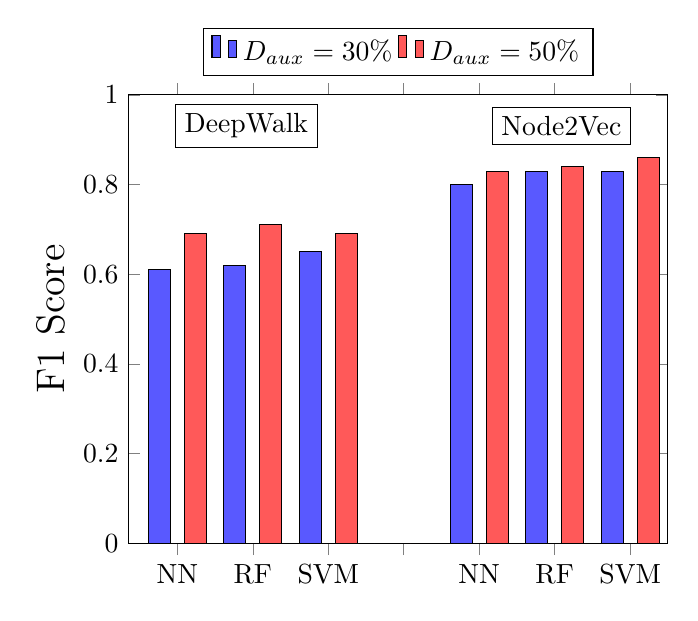
\begin{tikzpicture}
\begin{axis}[
ylabel=F1 Score,
%ylabel style={yshift=-1cm},
%xlabel=Architectures,
xtick={0,1,2,3,4,5,6,7},
xticklabels={,NN,RF,SVM,,NN,RF,SVM},
%xlabel style={yshift=0.35cm},
legend style={at={(0.5,1.15)},anchor=north,legend columns=-1,font=\normalsize},
ybar=5pt,% configures ‘bar shift’
bar width=8pt,
ylabel near ticks,
xlabel near ticks,
x label style={font=\Large},
y label style={anchor=south,font=\Large},
ytick style={font=\large},
xtick style={font=\large},
xmax=7.5,
ymin=0,
ymax=1
]

\addplot [fill=blue!65]
coordinates {(1,0.61) (2,0.62) (3,0.65) (4,0.0) (5,0.80) (6,0.83) (7,0.83)};
\addplot [fill=red!65]
coordinates {(1,0.69) (2,0.71) (3,0.69) (4,0.0) (5,0.83) (6,0.84) (7,0.86)};

\legend{$D_{aux}=30\%$, $D_{aux}=50\%$}
\end{axis}

\node[draw] at (5.5,5.3) {Node2Vec};
\node[draw] at (1.5,5.3) {DeepWalk};

\end{tikzpicture}



\end{document}
